\chapter{Implementazione del server}

Il server federato è il cuore del sistema; esso si occupa di ricevere i dati dai dispositivi embedded, di elaborarli e di inviarli ai client che ne fanno richiesta.

Esso è stato implementato in modo tale da essere scalabile, sicuro e in grado di gestire un gran numero di dispositivi connessi simultaneamente.

\section{Framework Web}

Come già accennato in precedenza (vedi capitolo 5.1.8), il server federato è stato sviluppato utilizzando il framework web Rocket, scritto interamente in Rust.
Grazie ad un ampio uso di macro a compile-time, Rocket è in grado di generare codice efficiente e sicuro,
serializzare e deserializzare automaticamente i dati in formato JSON e gestire le richieste HTTP in modo asincrono.
L'autenticazione e l'autorizzazione degli utenti sono gestite tramite un sistema di middleware che permette di definire rotte protette da token JWT.

\section{Struttura del progetto}

Il progetto del server federato è stato organizzato in maniera modulare; ciascuno 
dei moduli incapsula funzionalità specifiche necessarie per il funzionamento del server:

\begin{itemize}
    \item \texttt{main}: inizializza il server e avvia i task principali.
    \item \texttt{mailbox}: gestisce la coda dei messaggi in arrivo, distribuendoli ai client.
    \item \texttt{socket}: si occupa della comunicazione WebSocket con i dispositivi embedded.
    \item \texttt{db}: gestisce il database e contiene le strutture dati principali.
    \item \texttt{auth}: gestisce l'autenticazione e l'autorizzazione degli utenti tramite JWT.
    \item \texttt{cors}: fornisce un middleware per gestire le richieste cross-origin.
\end{itemize}

\section{Analisi dei moduli}

Analizziamo di seguito il codice dei moduli principali del server federato.

\subsection{main}

\begin{listing}[H]
    \begin{minted}[
        frame=single,
        framerule=0.8pt,
        fontsize=\footnotesize,
        breaklines
      ]{rust}
      #[launch]
      async fn rocket() -> _ {
        dotenv().ok();
        let db = Database::new("db");
        let (mut mailserver, tx) = MailServer::new();
        tokio::spawn(async move { mailserver.run().await });
        rocket::build()
            .attach(cors::Cors)
            .manage(db)
            .manage(Arc::new(Mutex::new(tx)))
            .mount(
                "/",
                routes![
                    me,
                    register,
                    login,
                    devices,
                    new_device,
                    socket::handle_ws,
                    cors::options,
                    ...
                ],
            )
    }
    \end{minted}
\end{listing}

La funzione \texttt{rocket} è l'entry point del server federato. Essa inizializza il database, la coda dei messaggi e il server Rocket.
Il crate \texttt{dotenv} è utilizzato per caricare le variabili d'ambiente dal file \texttt{.env} permettendo così di configurare il server senza doverne ricompilare il codice.
Il database è inizializzato con il path della cartella in cui verranno salvati i dati.

\subsection{mailbox}

\begin{listing}[H]
    \begin{minted}[
        frame=single,
        framerule=0.8pt,
        fontsize=\footnotesize,
        breaklines
      ]{rust}
    pub struct Mail {
        pub from: String,
        pub message: String,
    }

    struct MailBox {
        messages: Vec<Mail>,
        tx: tokio::sync::mpsc::Sender<Vec<Mail>>,
    }

    pub enum MailCommand {
        OpenBox(String, tokio::sync::mpsc::Sender<Vec<Mail>>),
        // To, Message
        Send(String, Mail),
        Receive(String),
    }

    pub struct MailServer {
        mailboxes: HashMap<String, MailBox>,
        rx: tokio::sync::mpsc::Receiver<MailCommand>,
    }
    \end{minted}
\end{listing}

Il modulo \texttt{mailbox} contiene le strutture dati necessarie per la gestione della coda dei messaggi.
\texttt{Mail} rappresenta un messaggio contenente il mittente e il testo.
\texttt{MailBox}  presente una lista di messaggi e un canale di comunicazione asincrono per l'invio.
\texttt{MailCommand} comprende i comandi che possono essere inviati alla coda dei messaggi.
\texttt{MailServer} include una hashmap di Mailboxes e un canale di comunicazione asincrono per ricevere i comandi.

\begin{listing}[H]
    \begin{minted}[
        frame=single,
        framerule=0.8pt,
        fontsize=\footnotesize,
        breaklines
      ]{rust}
    pub async fn run(&mut self) {
        while let Some(command) = self.rx.recv().await {
            match command {
                // Open a new mailbox ( or set the existing one to the new tx )
                MailCommand::OpenBox(name, tx) => {
                    let messages = if self.mailboxes.contains_key(&name) {
                        self.mailboxes.get_mut(&name).unwrap().messages.clone()
                    } else {
                        vec![]
                    };
                    self.mailboxes.insert(name, MailBox { messages, tx });
                }
                // Receive all messages in the mailbox
                MailCommand::Receive(name) => {
                    let mailbox = self
                        .mailboxes
                        .get_mut(&name)
                        .expect("Mailbox not found on receive");
                    if mailbox.messages.is_empty() {
                        continue;
                    }
                    mailbox.tx.send(mailbox.messages.clone()).await.unwrap();
                    mailbox.messages.clear();
                }
                // Attempt to send a message to the mailbox in a non-blocking way
                MailCommand::Send(to, message) => {
                    if !self.mailboxes.contains_key(&to) {
                        let _ = self.create_mailbox(to.clone());
                        // Receiver is created but not used
                        // This causes the mailbox to be created but try_send will fail
                    }
                    let mailbox: &mut MailBox = self.mailboxes.get_mut(&to).unwrap();
                    mailbox.messages.push(message);
                    if mailbox.tx.try_send(mailbox.messages.clone()).is_ok() {
                        mailbox.messages.clear();
                    }
                }
            }
        }
    }
    \end{minted}
\end{listing}

La funzione \texttt{run} del \texttt{MailServer} è un task asincrono che gestisce i comandi inviati alla coda dei messaggi.
Attraverso il pattern matching vengono gestiti i comandi \texttt{OpenBox}, \texttt{Receive} e \texttt{Send}.
\texttt{OpenBox} apre una nuova mailbox o aggiorna quella esistente, imposta il canale di comunicazione e invia i messaggi in coda.
\texttt{Receive} invia tutti i messaggi presenti nella mailbox al client in maniera asincrona.
\texttt{Send} invia un messaggio alla mailbox specificata, se esiste, altrimenti crea una nuova mailbox.

Il design pattern utilizzato è l' \textit{Inbox and outbox pattern}, ampiamente utilizzato in sistemi 
federati come ActivityPub poiché esso si adatta perfettamente a gestire anche la comunicazione
asincrona tra i vari nodi e si assicura che i messaggi vengano consegnati in modo affidabile.

\subsection{socket}

\begin{listing}[H]
    \begin{minted}[
        frame=single,
        framerule=0.8pt,
        fontsize=\footnotesize,
        breaklines
      ]{rust}
    #[get("/ws/<device_name>")]
    pub async fn handle_ws(
        tx: &State<Arc<Mutex<Sender<MailCommand>>>>,
        db: &State<Database>,
        ws: ws::WebSocket,
        device_name: String,
    ) -> ws::Channel<'static> {
        let device = db.devices.get(&device_name).unwrap().unwrap();
        let tx = tx.lock().await.clone();
        ws.channel(move |mut stream| {
            Box::pin(async move {
                // Send a challenge to the device
                let mut challenge = [0u8; 128];
                rand::thread_rng().fill(&mut challenge);
                stream
                    .send(encrypt(challenge.to_vec(), device.pub_key).into())
                    .await
                    .unwrap();
                // Wait for the response
                let response = stream.next().await.unwrap().unwrap();
                // Check if the response is correct
                if response.into_data() != challenge {
                    stream.send("Authentication error".into()).await.unwrap();
                    return Err(ws::result::Error::ConnectionClosed);
                }
    \end{minted}
\end{listing}

La funzione asincrona \texttt{handle\_ws} gestisce la comunicazione WebSocket con i dispositivi embedded e gli 
emulatori. Essa riceve il nome del dispositivo e lo autentifica tramite una challenge-response ovvero
crea una challenge casuale, la invia al dispositivo, attende la risposta e infine la confronta con la challenge originale.

\begin{listing}[H]
    \begin{minted}[
        frame=single,
        framerule=0.8pt,
        fontsize=\footnotesize,
        breaklines
      ]{rust}
                let (my_tx, mut my_rx) = tokio::sync::mpsc::channel::<Vec<Mail>>(32);

                tx.send(MailCommand::OpenBox(device_name.clone(), my_tx))
                    .await
                    .unwrap();

                loop {
                    tx.send(MailCommand::Receive(device_name.clone()))
                        .await
                        .unwrap();
                    select! {
                        message = stream.next() => {
                            if let Some(Ok(message)) = message {
                                let new_mail: NewMail = json::from_slice(&message.into_data())
                                                        .unwrap();
                                tx.send(MailCommand::Send(new_mail.to.clone(), Mail {
                                    from: device_name.clone(),
                                    message: new_mail.message,
                                })).await.unwrap();
                            } else {
                                break;
                            }
                        }
                        message = my_rx.recv() => {
                            dbg!(&message);
                            stream.send(json::json!{
                                message.unwrap()
                            }.to_string().into()).await.unwrap();
                        }
                    }
                }
                Ok(())
            })
        })
    }
    \end{minted}
\end{listing}

La restante parte della funzione si occupa l'invio e la ricezione dei messaggi tra il dispositivo e il server federato
utilizzando il sistema di messaggistica implementato nel modulo \texttt{mailbox}.

\subsection{db}

\begin{figure}[H]
    \centering
    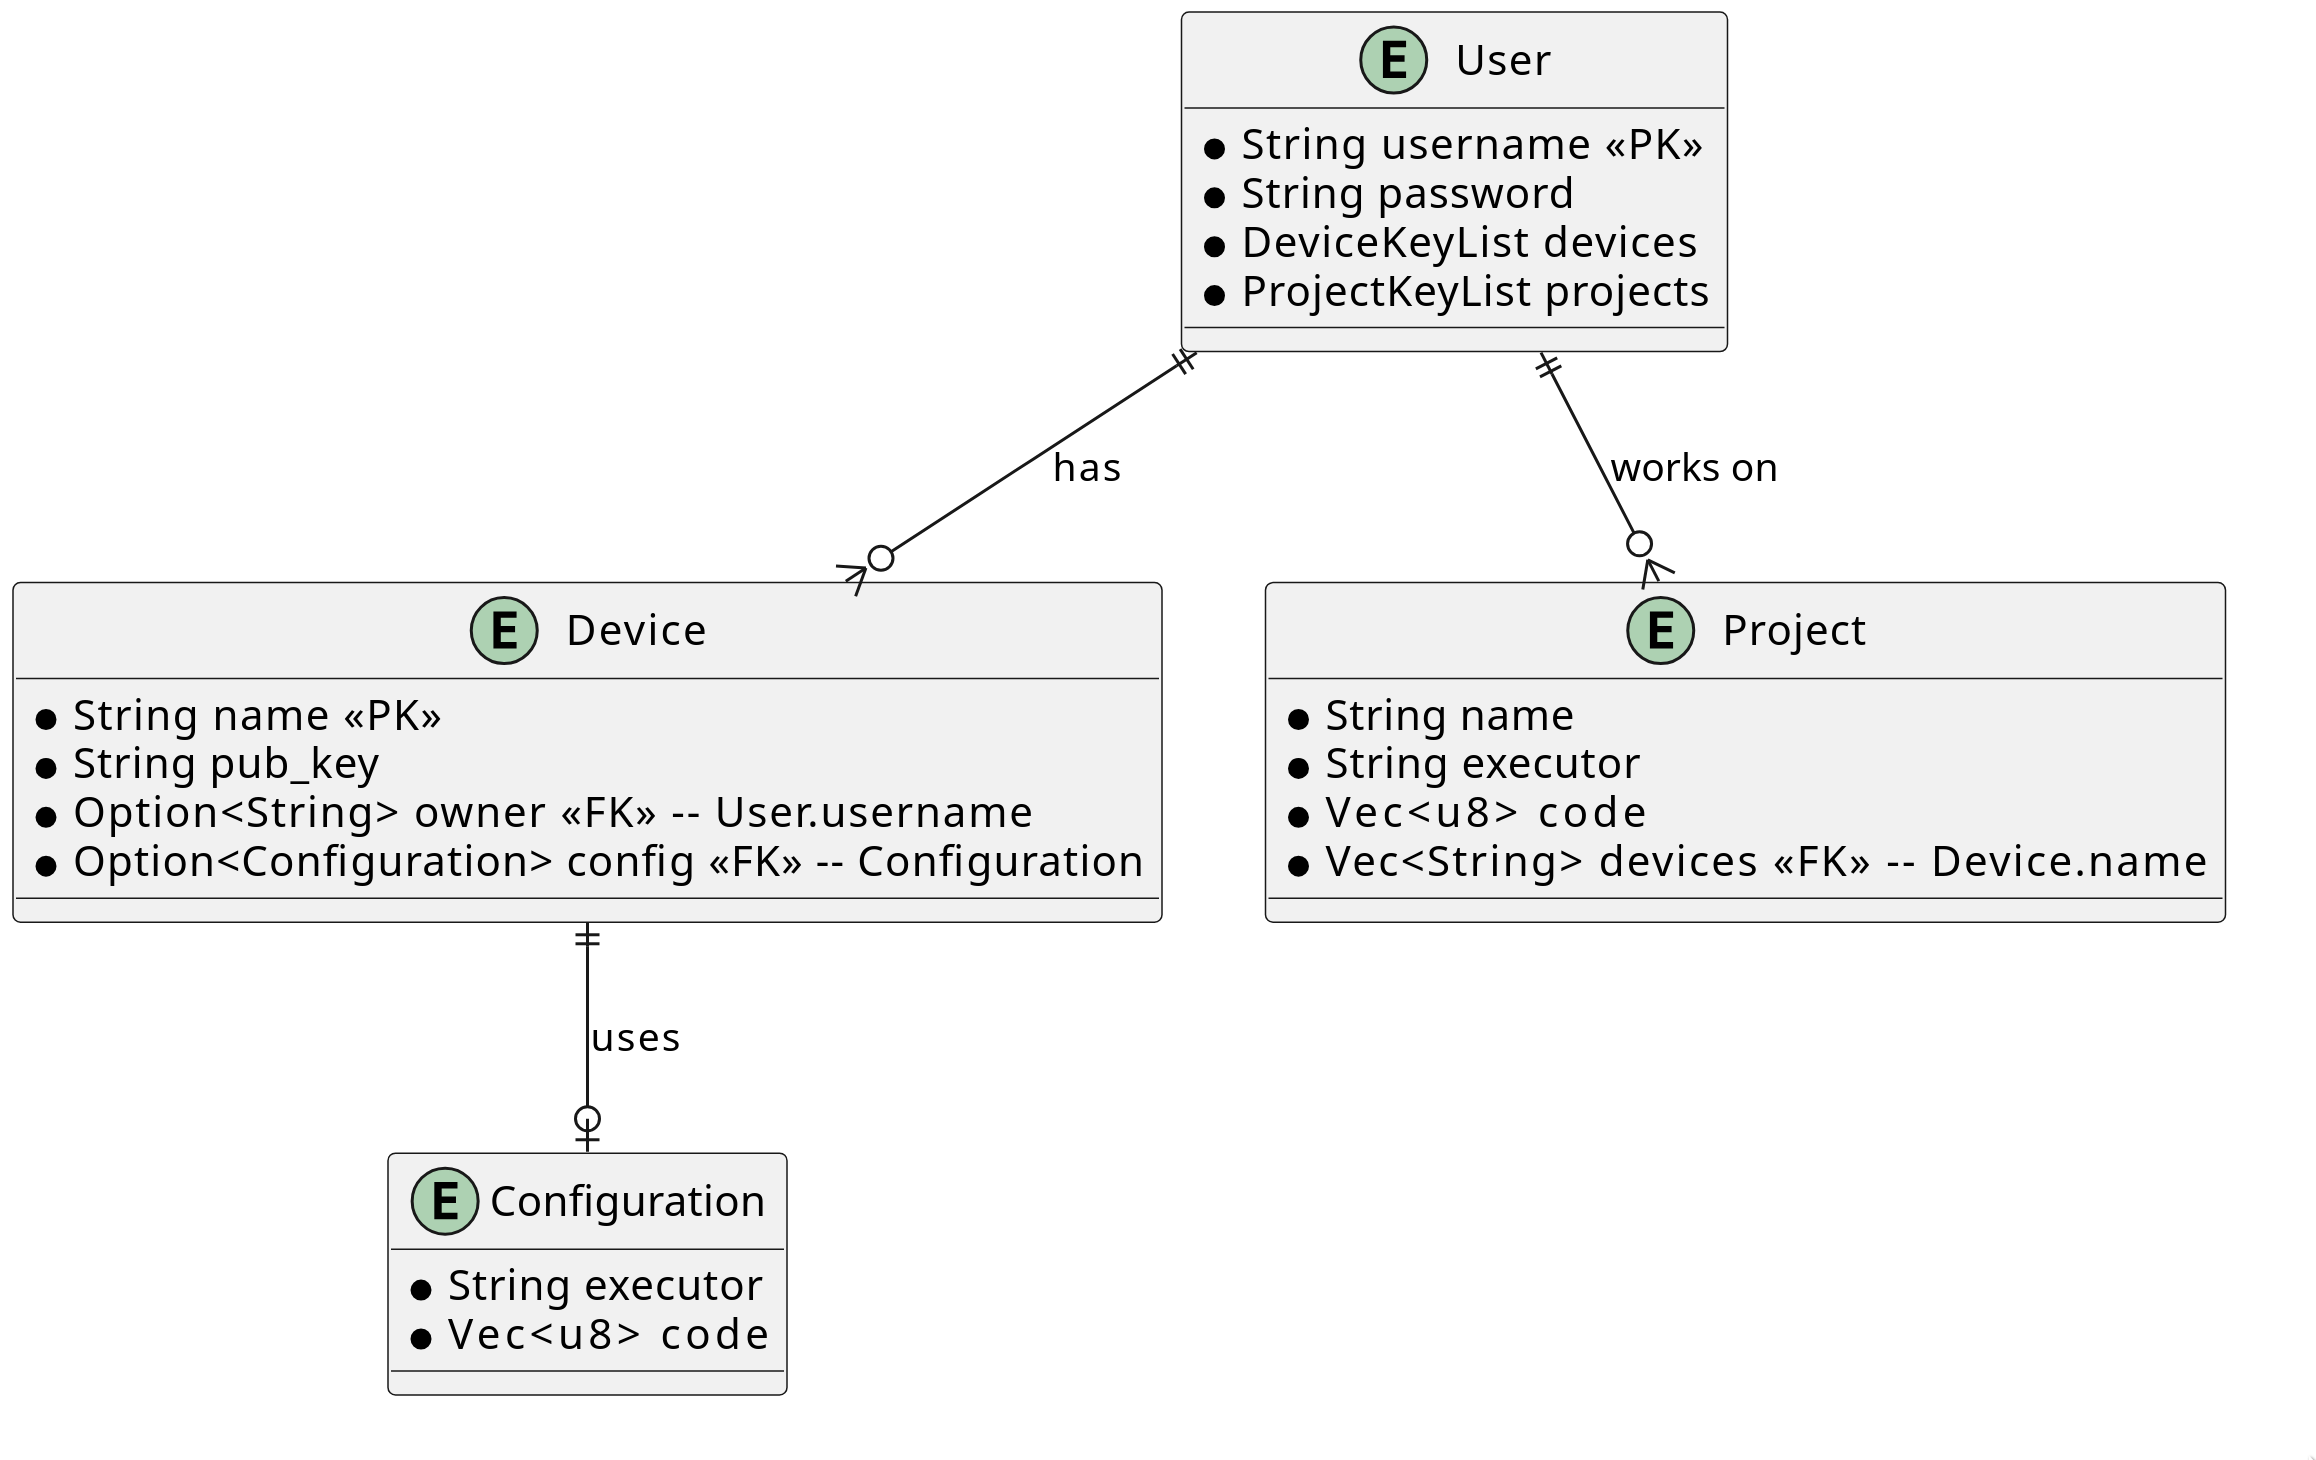
\includegraphics[width=0.8\textwidth]{images/chapter6/uml-db.png}
    \caption{ Schema UML del database }
    \label{fig:blender}
  \end{figure}

\begin{listing}[H]
    \begin{minted}[
        frame=single,
        framerule=0.8pt,
        fontsize=\footnotesize,
        breaklines
      ]{rust}
    pub struct Database {
        pub db: Db,
        pub users: Tree<String, User>,
        pub devices: Tree<String, Device>,
        // Project keys are stored as (username, project_name)
        pub projects: Tree<(String, String), Project>,
    }
\end{minted}
\end{listing}

Il modulo \texttt{db} contiene la struttura dati \texttt{Database} che rappresenta il database del server federato.
Il database è implementato utilizzando il crate \texttt{sled}, un database key-value embedded in Rust e contiene tre \texttt{Tree}:
\texttt{users}, \texttt{devices} e \texttt{projects} che si riferiscono rispettivamente gli utenti, i dispositivi e i progetti.

\subsection{auth}

\begin{listing}[H]
    \begin{minted}[
        frame=single,
        framerule=0.8pt,
        fontsize=\footnotesize,
        breaklines
      ]{rust}
    #[derive(Serialize, Deserialize, Debug)]
    pub struct Claim {
        pub username: String,
        exp: u64,
    }
    \end{minted}
\end{listing}

Il modulo \texttt{auth} contiene la struttura dati \texttt{Claim} che rappresenta il token JWT.
Il claim, formato dal nome utente e data di scadenza, viene 
generato e firmato in maniera sicura dal server al momento del login.

\begin{listing}[H]
    \begin{minted}[
        frame=single,
        framerule=0.8pt,
        fontsize=\footnotesize,
        breaklines
      ]{rust}
    #[rocket::async_trait]
    impl<'r> FromRequest<'r> for Claim {
        type Error = String;

        async fn from_request(req: &'r Request<'_>) -> request::Outcome<Self, Self::Error> {
            match req.headers().get_one("authorization").and_then(decode_jwt) {
                Some(claim) => rocket::outcome::Outcome::Success(claim),
                None => {
                    rocket::outcome::Outcome::Error((Status::Unauthorized, "Invalid JWT".to_string()))
                }
            }
        }
    }
    \end{minted}
\end{listing}


Il client dovrà includere il token JWT nell'header delle richieste HTTP per autenticarsi e accedere alle rotte protette,
necessario per la verifica del claim da parte del server.
La struttura dati \texttt{Claim} implementa infatti il trait \texttt{FromRequest} di Rocket
consentendo di definire un middleware per la verifica automatica del token.

\subsection{cors}

\begin{listing}[H]
    \begin{minted}[
        frame=single,
        framerule=0.8pt,
        fontsize=\footnotesize,
        breaklines
      ]{rust}
    #[rocket::async_trait]
    impl Fairing for Cors {
        fn info(&self) -> Info {
            Info {
                name: "Add CORS headers to responses",
                kind: Kind::Response,
            }
        }

        async fn on_response<'r>(&self, _request: &'r Request<'_>, response: &mut Response<'r>) {
            response.set_header(Header::new("Access-Control-Allow-Origin", "*"));
            response.set_header(Header::new(
                "Access-Control-Allow-Methods",
                "POST, GET, PATCH, OPTIONS, DELETE, PUT",
            ));
            response.set_header(Header::new("Access-Control-Allow-Headers", "*"));
            response.set_header(Header::new("Access-Control-Allow-Credentials", "true"));
        }
    }
    \end{minted}
\end{listing}

Il modulo \texttt{cors} fornisce un Fairing~\cite{rocket_fairing} per gestire le richieste cross-origin
e consente ai client di effettuare richieste HTTP da domini diversi.